\chapter{ As medidas de desempenho de uma operação de produção} 
\label{chap:medida_desempenho_operacao_prod} 

\section{Medidas de desempenho} 
\label{sec:sistemas_produtivos_desempenho} 
Para medir corretamente o desempenho de uma operação produtiva é necessário o uso de certos indicadores. Para isso, foi desenvolvido o sistema chamado \textit{Balanced Scorecard (BSC)}, este é utilizado por ser considerado o mais equilibrado na aferição dos indicadores de desempenho da operação.
Na Figura \ref{fig:balanced_scorecard}, uma versão adaptada do BSC, baseado nos indicadores:

\begin{itemize}
    \item Financeiros: Maior importância para proprietários e sócios da empresa;
    \item De percepção do cliente: A opinião do cliente sobre a empresa e o produto;
    \item De processos internos: A comparação com os parâmetros operacionais a serem analisados;
    \item De aprendizagem e crescimento: A competência de manter-se sustentável através de aprendizado, mudanças e melhoras ao longo do tempo.  
\end{itemize}


\begin{figure}[H]
    \centering
    \caption{Balanced Scorecard (BSC)}
    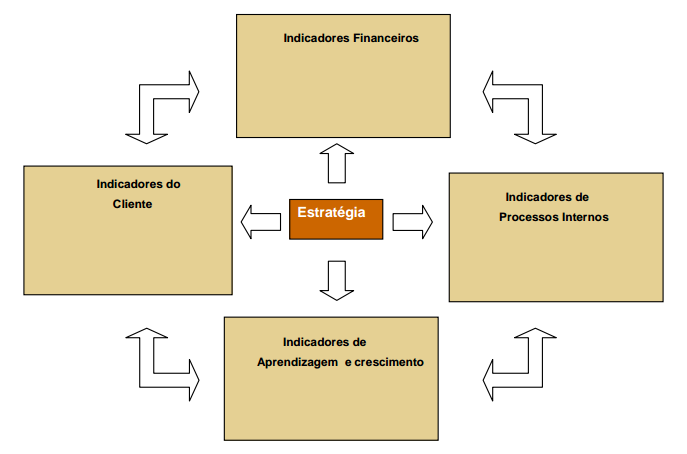
\includegraphics[width =0.8\textwidth]{images/bsc.png}
    \caption*{Fonte: Adaptado de \cite{kaplan1996using}}
    \label{fig:balanced_scorecard}
\end{figure}

O BSC é um sistema de medição de origem estratégica e seus indicadores são escolhidos de acordo com as necessidades atuais da empresa. Com o uso do sistema é esperado que se atinja o aprimoramento contínuo do negócio ao mesmo tempo que se tenha uma preocupação constante com o aprendizado e adaptação, estabelecendo novas metas para uma melhoria contínua.

Outro ponto importante a ser discutido é a diferença entre eficácia e eficiência. A primeira, representa a conquista de objetivos enquanto eficiência é a maneira como estes objetivos são atingidos. A interpretação destes dois parâmetros de medição, é imprescindível e indissociável para a gestão de uma operação produtiva.

Reconhecendo relevância de se medir o desempenho e entendendo a real diferença entre eficácia e eficiência, devemos listar os principais objetivos de desempenho estratégico em uma empresa industrial. Slack (2006) cita cinco objetivos gerais de desempenho. São eles: Qualidade, Velocidade, Flexibilidade, Confiabilidade e Custo. 

\section{Aplicação Prática} 
\label{sec:estrategia_da_producao_aplicacao}


